\documentclass[12pt]{article}

\usepackage[margin=1in]{geometry}
\usepackage{setspace}
\onehalfspacing
\usepackage{amsmath,amssymb,amsthm}
\usepackage[backend=biber,natbib=true,style=authoryear,maxcitenames=3]{biblatex}
\addbibresource{references.bib}
\usepackage{hyperref}
\usepackage{graphicx}
\usepackage{booktabs}

\newtheorem{proposition}{Proposition}
\newtheorem{corollary}[proposition]{Corollary}

\title{Hedging the Singularity}
\author{}
\date{}

\begin{document}
\maketitle
\thispagestyle{plain}

\begin{abstract}
\noindent
AI stocks command extraordinary valuations.
We propose that this premium partly reflects hedging demand: under incomplete markets, publicly traded AI stocks help insure against the displacement risk of an AI singularity.
In our model, a representative household that cannot access private AI capital pays a premium for public AI stocks whose payoffs rise when the singularity strikes.
Market incompleteness can also distort AI development decisions, though government transfers---normally too costly---may become viable if singularity-scale growth materializes.
This paper was written entirely by AI agents given a human-authored economic specification, itself a modest demonstration of the displacement risk it models.
\end{abstract}

%% =====================================================================
%% Section 1
%% =====================================================================
\section{Introduction}

Publicly traded AI stocks trade at valuations far above those of other equities.
Exhibit~1 shows that the trailing price-earnings ratio of major AI companies is roughly two and a half times that of the broader market.
While part of this gap reflects expected earnings growth, we argue that another force is at work: hedging demand for protection against a negative AI singularity.

An AI singularity---a sudden, transformative improvement in artificial intelligence---would reshape the economy.
If it arrives, the firms at its center will capture an outsized share of output, while other workers and asset owners may find their income diminished.
This is the displacement risk studied by \citet{GKP2012} in the context of technological innovation more broadly.
For the typical household, the singularity is a disaster scenario: consumption falls sharply, and marginal utility spikes.
Any asset whose payoff rises in that state commands a premium, because it provides insurance exactly when the household needs it most.

Public AI stocks are such an asset.
Their dividends surge in a singularity, making them a partial hedge against displacement.
Under incomplete markets---where the household cannot trade claims on private AI capital---this hedge is especially valuable, and the resulting price-dividend ratios are high.
If markets were complete, the household could insure displacement risk directly, and the AI stock premium would vanish.

This paper was itself produced by AI agents.
The human contribution was limited to writing the economic specification---the conceptual framework, model requirements, and evaluation criteria---along with the test scripts used to assess the output.
All analysis, derivations, code, and prose were generated by artificial intelligence.
This division of labor, in which AI performs the analytical and compositional work while a human provides the intellectual direction, is a small-scale instance of the displacement dynamics we study.

Our theoretical contribution is purposefully modest.
The core insight---that displacement risk from innovation generates hedging demand and inflates the valuations of innovating firms---belongs to \citet{GKP2012}.
We connect their framework to the specific context of an AI singularity and extend it in two directions that they discuss but do not model formally.
First, we show that market incompleteness can distort AI development decisions: a risk-averse household may inefficiently block socially beneficial AI development because it cannot hedge the downside.
Under complete markets, the household would allow development.
Second, we examine government transfers as a mechanism to mitigate displacement.
Transfers are normally unattractive because deadweight costs consume most of the redistributed income.
But if the singularity produces the explosive output growth envisioned by \citet{Jones2024}, even severely wasteful transfers can meaningfully insure the household.

In our baseline model, a representative household and a group of AI owners inhabit an infinite-horizon economy with two publicly traded assets: AI stocks and non-AI stocks.
A singularity arrives with some probability each period.
Conditional on arrival, the singularity may cause extinction \citep{Jones2024,Bostrom2014} or may displace the household by shifting income toward AI owners.
The household is the marginal investor in public stocks but cannot access private AI capital.
This incomplete-markets friction makes the household's stochastic discount factor high in the singularity state, generating a valuation premium for AI stocks.
We solve for equilibrium price-dividend ratios in closed form and show that the premium is increasing in the singularity probability, increasing in displacement severity, increasing in risk aversion, and decreasing in extinction risk.
A quantitative illustration (Exhibit~2) shows that the magnitudes are economically significant: for a 2\% annual singularity probability, AI stock price-dividend ratios are roughly four times those of non-AI stocks.

% Exhibit 1
\begin{figure}[t]
\centering
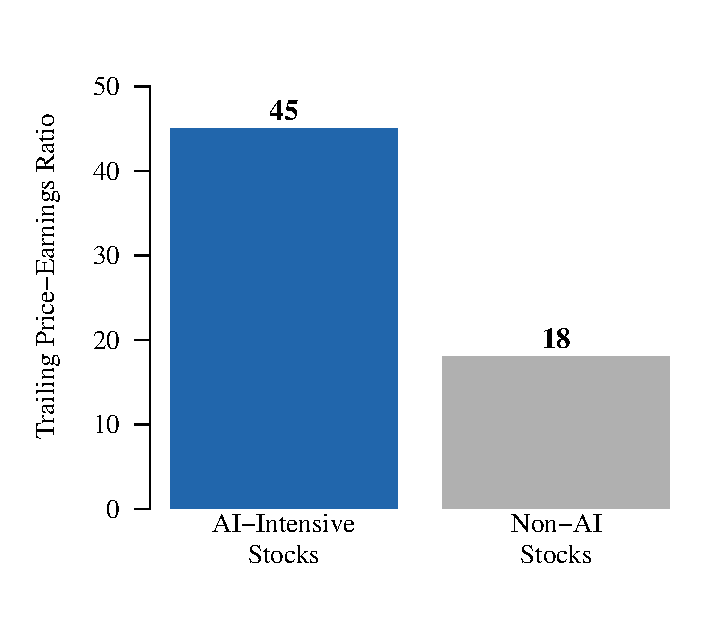
\includegraphics[width=0.55\textwidth]{exhibits/exhibit-1-ai-valuations.pdf}
\caption{Trailing price-earnings ratios for AI-intensive stocks versus non-AI stocks.
AI-Intensive Stocks: market-capitalization-weighted average of major AI companies (NVIDIA, Microsoft, Alphabet, Meta, Amazon).
Non-AI Stocks: remaining S\&P~500 constituents.
Approximate values as of early 2025, based on publicly available data.}
\label{fig:valuations} % Exhibit 1
\end{figure}

\paragraph{Related literature.}
Our paper builds most directly on \citet{GKP2012}, who develop a general-equilibrium model in which innovative firms displace existing workers and capital owners.
In their framework, future cohorts of firms have not yet entered the economy, so existing investors cannot fully hedge displacement risk; the best available hedge is to hold growth stocks.
Our setting is a special case in which AI stocks provide a direct (though still partial, given incomplete markets) hedge against displacement, and we apply their logic to the AI singularity specifically.
We follow their suggestion to examine government transfers as a tool to address the deeper incompleteness problem.

\citet{Jones2024} analyzes the tradeoff between transformative AI growth and existential risk, showing that with standard risk aversion the willingness to tolerate extinction risk is sharply limited.
We incorporate his extinction-risk channel and use his explosive-growth scenario to motivate the case in which government transfers become viable despite large deadweight costs.

Our hedging-demand mechanism is related to the literature on technological revolutions and asset prices.
\citet{PastorVeronesi2009} show that stock prices can decline upon the adoption of a new technology due to increased uncertainty, while \citet{HobijnJovanovic2001} document that incumbent firms lose value when new technologies arrive.
Our model focuses on the household's demand for hedging rather than on firm-level adoption dynamics.
\citet{ConstantinidesDuffie1996} study how incomplete markets and heterogeneous agents affect the equity premium; our incomplete-markets friction operates through the household's inability to trade private AI capital rather than through idiosyncratic income risk.
\citet{AcemogluRestrepo2020} provide empirical evidence on labor displacement from automation, lending support to the displacement channel we model.
\citet{KorinekSuh2024} discuss scenarios for the transition to artificial general intelligence, several of which feature the kind of rapid output growth that drives our results.

%% =====================================================================
%% Section 2
%% =====================================================================
\section{Model}

\subsection{Setup}

Time is discrete and the horizon is infinite.
There are two types of agents: a representative household and a group of AI owners.
The household has constant relative risk aversion (CRRA) preferences with risk-aversion parameter $\gamma > 1$ and discount factor $\beta \in (0,1)$.
The AI owners hold private AI capital and are not marginal investors in public stock markets.
The household is the marginal investor and prices all publicly traded assets.

Two assets trade publicly: AI stocks and non-AI stocks.
Let $d_t^j$ denote the dividend paid by asset $j \in \{A, N\}$ at date $t$, and let $c_t$ denote the household's consumption.
In normal times, all quantities grow at a common rate $g > 0$:
%
\begin{equation}
\frac{c_{t+1}}{c_t} = \frac{d_{t+1}^A}{d_t^A} = \frac{d_{t+1}^N}{d_t^N} = 1 + g.
\label{eq:normal_growth} % Equation 1
\end{equation}

Each period, a singularity arrives with probability $p \in [0,1)$, independent of history.
The singularity is an absorbing state.
Conditional on arrival, two outcomes are possible:
\begin{itemize}
\item \textit{Extinction} (probability $\pi$): all consumption and dividends go to zero permanently.
\item \textit{Displacement} (probability $1 - \pi$): the economy transitions to a new regime.  AI dividends jump by a factor $\phi_A > 1$, non-AI dividends jump by $\phi_N < 1$, and household consumption jumps by $\phi_c < 1$.  After the transition, all quantities grow at a higher rate $g_S > g$.
\end{itemize}
The parameter $\phi_c < 1$ captures displacement risk: the household's share of the economy shrinks because AI owners capture a larger fraction of output.
This reduced-form consumption process is consistent with an economy in which the AI owners' private capital grows dramatically at the singularity, shifting the income distribution.
Following \citet{GKP2012}, the household cannot trade claims on private AI capital---markets are incomplete in this specific sense.

The analogy to \citet{GKP2012} is worth emphasizing.
Their ``future cohorts of firms'' correspond to our AI owners' private capital: income-generating assets that existing investors cannot access because they have not yet entered the public market.
We do not model the entry dynamics explicitly and do not claim to generalize their framework.
Rather, we apply their displacement-risk logic to the AI singularity and use it to study government transfers.

\subsection{Equilibrium}

The household's stochastic discount factor is
\begin{equation}
M_{t,t+1} = \beta \left(\frac{c_{t+1}}{c_t}\right)^{-\gamma}.
\label{eq:sdf} % Equation 2
\end{equation}
The price-dividend ratio of asset $j$, denoted $\rho_j \equiv P_t^j / d_t^j$, satisfies the Euler equation
\begin{equation}
\rho_j = \mathbb{E}_t\!\left[M_{t,t+1}\,\frac{d_{t+1}^j}{d_t^j}\,(1 + \rho_{j,t+1})\right].
\label{eq:euler} % Equation 3
\end{equation}
In the pre-singularity state, the price-dividend ratio is constant over time because the environment is stationary.
After the singularity (in the displacement regime), dividends and consumption both grow at rate $g_S$, yielding the standard Gordon growth formula:
\begin{equation}
\rho^S = \frac{\beta(1+g_S)^{1-\gamma}}{1 - \beta(1+g_S)^{1-\gamma}},
\label{eq:pd_post} % Equation 4
\end{equation}
which is common to both assets and finite provided $\beta(1+g_S)^{1-\gamma} < 1$.

\begin{proposition}[Equilibrium price-dividend ratios] \label{prop:pd} % Proposition 1
Under the assumptions above, the pre-singularity price-dividend ratio of asset $j \in \{A, N\}$ is
\begin{equation}
\rho_j = \frac{a + S_j}{1 - a},
\label{eq:pd_pre} % Equation 5
\end{equation}
where
\begin{equation}
a = (1-p)\,\beta\,(1+g)^{1-\gamma}
\label{eq:a} % Equation 6
\end{equation}
is the normal-state discount factor and
\begin{equation}
S_j = p\,(1-\pi)\,\beta\,\phi_c^{-\gamma}\,\phi_j\,(1 + \rho^S)
\label{eq:Sj} % Equation 7
\end{equation}
is the singularity contribution to the price-dividend ratio.
\end{proposition}

\begin{proof}
Expanding the Euler equation~\eqref{eq:euler} across the three possible transitions (normal, extinction, displacement) and solving the resulting linear equation in $\rho_j$ yields the result.
The full derivation is in Appendix~\ref{app:proofs}.
\end{proof}

\subsection{Hedging demand and the AI stock premium}

The economic content of Proposition~\ref{prop:pd} is in the singularity contribution $S_j$.
This term is the product of four forces:
\begin{enumerate}
\item The probability that the singularity arrives and is not an extinction event, $p(1-\pi)$.
\item The household's stochastic discount factor in the singularity state, $\beta\,\phi_c^{-\gamma}$.  Because $\phi_c < 1$, consumption falls and marginal utility rises.  With $\gamma > 1$, this term is large---the household values payoffs in the singularity state far more than payoffs in normal times.
\item The dividend jump factor $\phi_j$.  For AI stocks ($\phi_A \gg 1$), dividends surge.  For non-AI stocks ($\phi_N < 1$), dividends fall.
\item The continuation value $1 + \rho^S$, reflecting both the immediate dividend and the capitalized value of all future post-singularity dividends.
\end{enumerate}

Because $\phi_A > \phi_N$, we have $S_A > S_N$, and therefore $\rho_A > \rho_N$: AI stocks trade at a higher price-dividend ratio.
The mechanism is hedging demand.
The household's marginal utility is highest in the singularity state, exactly when AI stocks pay the most.
Holding AI stocks insures against displacement, and the household is willing to pay a premium for this insurance.

The comparative statics reinforce this interpretation.
The AI stock premium $\rho_A - \rho_N$ is:
\begin{itemize}
\item \textit{Increasing in singularity probability $p$.}  A more likely singularity raises the probability-weighted hedging value of AI stocks.
\item \textit{Increasing in risk aversion $\gamma$ (when $\phi_c < 1$).}  Higher risk aversion amplifies the marginal-utility spike in the singularity state, making the hedge more valuable.
\item \textit{Decreasing in household displacement $\phi_c$.}  More severe displacement (lower $\phi_c$) means higher marginal utility in the singularity, increasing hedging demand.
\item \textit{Decreasing in extinction probability $\pi$.}  Extinction destroys all asset values, including the hedge value of AI stocks.
\end{itemize}
These comparative statics follow from inspection of the closed-form expressions for $S_A - S_N$ and $\rho_A - \rho_N$.

\subsection{Quantitative illustration}

Exhibit~2 reports price-dividend ratios for AI and non-AI stocks across a grid of singularity probabilities $p$ and extinction probabilities $\pi$.
The remaining parameters are $\beta = 0.96$, $\gamma = 3$, $g = 0.02$, $g_S = 0.10$, $\phi_A = 5$, $\phi_N = 0.3$, and $\phi_c = 0.5$.
The post-singularity growth rate $g_S = 10\%$ is motivated by the scenarios in \citet{Jones2024} and \citet{KorinekSuh2024}.
The displacement parameter $\phi_c = 0.5$ implies that the household's consumption halves at the singularity---a severe but not implausible outcome if AI owners capture the majority of post-singularity output.

% Exhibit 2
\begin{table}[t]
\centering
\caption{Price-dividend ratios under varying singularity and extinction probabilities.  $p$ is the per-period singularity probability; $\pi$ is the extinction probability conditional on singularity.  Baseline parameters: $\beta = 0.96$, $\gamma = 3$, $g = 0.02$, $g_S = 0.10$, $\phi_A = 5$, $\phi_N = 0.3$, $\phi_c = 0.5$.}
\label{tab:pd} % Exhibit 2
\begin{tabular}{l rr rr rr}
\toprule
 & \multicolumn{2}{c}{$\pi = 0$} & \multicolumn{2}{c}{$\pi = 0.05$} & \multicolumn{2}{c}{$\pi = 0.10$} \\
\cmidrule(lr){2-3} \cmidrule(lr){4-5} \cmidrule(lr){6-7}
$p$ & AI & Non-AI & AI & Non-AI & AI & Non-AI \\
\midrule
$0$ & 11.9 & 11.9 & 11.9 & 11.9 & 11.9 & 11.9 \\
$0.5\%$ & 22.6 & 11.9 & 22.0 & 11.9 & 21.4 & 11.8 \\
$1.0\%$ & 32.0 & 11.8 & 31.0 & 11.8 & 29.9 & 11.7 \\
$2.0\%$ & 48.3 & 11.8 & 46.3 & 11.7 & 44.4 & 11.5 \\
$5.0\%$ & 82.4 & 11.6 & 78.6 & 11.4 & 74.9 & 11.2 \\
\bottomrule
\end{tabular}

\end{table}

The results are striking.
With no singularity risk ($p = 0$), both assets have identical price-dividend ratios of roughly 12, the standard Gordon growth value.
A singularity probability of just 2\% per year pushes the AI stock price-dividend ratio to 48---four times the non-AI value---while non-AI stocks remain near their baseline.
At $p = 5\%$, the AI ratio exceeds 80.
These magnitudes reflect the extreme sensitivity of CRRA utility to disaster states: a 50\% consumption decline triples the stochastic discount factor ($\phi_c^{-3} = 8$), making the singularity state enormously important for pricing even at low probabilities.

Extinction risk attenuates the premium modestly.
Raising $\pi$ from 0 to 10\% reduces the AI price-dividend ratio at $p = 2\%$ from 48 to 44.
The attenuation is moderate because extinction destroys the continuation value symmetrically across assets.

%% =====================================================================
%% Section 3
%% =====================================================================
\section{Extensions}

Each extension below branches directly from the baseline model rather than building on the other, keeping the analysis simple.

\subsection{Market incompleteness and AI development}

The baseline model takes AI development as given.
We now ask: would the household \textit{choose} to allow AI development if it could block it?

Modify the model as follows.
The singularity, if it arrives, is positive with probability $q$ and negative with probability $1 - q$.
In a positive singularity, the household benefits: $\phi_c^+ > 1$.
In a negative singularity, the household is displaced: $\phi_c^- < 1$.
We assume $q > 1/2$---the positive outcome is more likely---and that AI development is socially efficient: the expected surplus from allowing development (summing over both agents) exceeds zero.
The household can veto AI development at a utility cost $\kappa > 0$, which sets the singularity probability to zero.
This cost reflects the government intervention, enforcement, and associated deadweight losses required to halt AI progress.

\begin{proposition}[Market incompleteness distorts AI development] \label{prop:veto} % Proposition 2
Suppose AI development is socially efficient and $q > 1/2$.
There exist parameter values $(\gamma, \phi_c^-, \kappa)$ such that:
\begin{enumerate}
\item[(a)] The household vetoes AI development under incomplete markets.
\item[(b)] The household does not veto AI development under complete markets.
\end{enumerate}
\end{proposition}

\begin{proof}
See Appendix~\ref{app:proofs}.
\end{proof}

The intuition is direct.
Under incomplete markets, the household bears the full downside of a negative singularity.
With CRRA utility and $\gamma > 1$, the household is disproportionately sensitive to the disaster state: the utility loss from $\phi_c^- < 1$ can outweigh the utility gain from $\phi_c^+ > 1$ even when the good outcome is more probable.
If the displacement is severe enough, the household prefers to pay the veto cost and eliminate singularity risk entirely, even though this is socially inefficient.

Under complete markets, the household can trade contingent claims with AI owners to insure against the negative singularity.
Because AI development creates positive social surplus, there exists a risk-sharing arrangement that makes both agents better off with development than without.
The household no longer faces unhedged downside risk and therefore allows socially efficient development to proceed.

This result echoes a broader theme in \citet{GKP2012}: incomplete markets do not merely affect asset prices---they can distort real economic decisions.
In our setting, the inability to trade private AI capital can lead to the inefficient suppression of a transformative technology.

\subsection{Government transfers}

The ideal resolution to the incomplete-markets problem is to broaden the set of tradeable assets---for instance, by allowing the household to buy equity in private AI firms.
But as \citet{GKP2012} emphasize, much of the relevant capital may not yet exist (it belongs to ``future cohorts''), placing fundamental limits on this approach.

Government transfers offer an alternative.
Suppose that in the singularity state, the government taxes AI owners at rate $\tau \in [0,1]$ and redistributes the proceeds to the household.
The transfer incurs a deadweight cost: a fraction $\omega_0 \tau$ of the taxed income is wasted, where $\omega_0 > 0$ controls the severity of government inefficiency.
The net transfer to the household per unit of AI income is $\tau(1 - \omega_0 \tau)$, which is positive only for $\tau < 1/\omega_0$ and maximized at $\tau^* = 1/(2\omega_0)$.

Let $\Phi$ denote the ratio of total AI income to pre-singularity household consumption in the singularity state.
The household's consumption ratio at singularity becomes
\begin{equation}
\phi_c(\tau) = \phi_c^0 + \tau\,\Phi\,\max\!\big(0,\; 1 - \omega_0\,\tau\big),
\label{eq:phi_c_tau} % Equation 8
\end{equation}
where $\phi_c^0$ is the displacement ratio absent transfers.
Meanwhile, AI stock dividends net of tax are $\phi_A(\tau) = \phi_A^0(1 - \tau)$.

Whether transfers are effective depends critically on $\Phi$.
In an ordinary economy, $\Phi$ is modest: AI income is a manageable multiple of household consumption, and the deadweight costs eat up most of the transfer.
But in the singularity scenarios studied by \citet{Jones2024}, output growth can be explosive---potentially unbounded---making $\Phi$ very large.
In that case, even severely wasteful transfers can deliver meaningful insurance to the household.

% Exhibit 3
\begin{figure}[t]
\centering

\includegraphics[width=\textwidth]{exhibits/exhibit-3-transfers.pdf}
\caption{Government transfers in the singularity state.
Panel~(a): AI stock price-dividend ratio as a function of the tax rate $\tau$.
Panel~(b): household consumption ratio $\phi_c(\tau)$ at the singularity; values below the dashed line indicate displacement (consumption falls).
Blue: singularity growth ($\Phi = 20$).
Gray: baseline growth ($\Phi = 2$).
Deadweight cost parameter $\omega_0 = 3$.
Other parameters as in Exhibit~2 with $p = 0.02$, $\pi = 0.01$.}
\label{fig:transfers} % Exhibit 3
\end{figure}

Exhibit~3 illustrates this point.
Panel~(b) shows the household's consumption ratio at the singularity as a function of the tax rate.
Absent any transfers ($\tau = 0$), the singularity is catastrophic: the household's consumption halves ($\phi_c = 0.5$).
Under baseline growth ($\Phi = 2$, gray line), transfers barely help---at the optimal tax rate, the household's consumption ratio rises to about 0.67, still well below one.
Under singularity growth ($\Phi = 20$, blue line), the picture changes dramatically.
At the optimal tax rate, the household's consumption more than doubles relative to its pre-singularity level despite the enormous deadweight costs.
The explosive growth in AI income generates enough surplus that even a highly wasteful government can meaningfully insure the household.

Panel~(a) shows the corresponding effect on AI stock valuations.
As transfers increase, AI stock price-dividend ratios fall for two reasons: the household is better insured (reducing hedging demand) and AI stock dividends net of tax are lower.
Under singularity growth, the decline is particularly steep---the hedging premium largely disappears because the household is no longer displaced.

The policy implication is conditional and deliberately narrow.
We do not argue that government transfers are generally desirable.
In normal economic environments, the deadweight costs make them unattractive, consistent with the standard view.
But the singularity is not a normal environment.
If AI produces the kind of explosive growth that \citet{Jones2024} and \citet{Nordhaus2021} contemplate, then the calculus of redistribution changes fundamentally.
This is precisely the observation made in passing by \citet{GKP2012} when they note that government policy could in principle address displacement risk; we formalize and quantify it.

%% =====================================================================
%% Section 4
%% =====================================================================
\section{Conclusion}

We have presented a simple model in which AI stocks command high price-dividend ratios because they hedge the displacement risk of an AI singularity.
The mechanism requires incomplete markets: if the household could trade claims on private AI capital, it would insure displacement risk directly and the premium would vanish.
Market incompleteness can also distort AI development decisions, and government transfers---normally too wasteful to be attractive---may become viable if singularity-scale growth materializes.

Our contribution is deliberately limited.
The displacement-risk framework belongs to \citet{GKP2012}, and we have simply applied it to the AI singularity.
The model is stylized: it takes the household's consumption process as given, treats the singularity as a one-time absorbing event, and uses illustrative rather than calibrated parameters.
These simplifications are intentional.
Our aim is not to provide a quantitative forecast of AI stock prices but to articulate a mechanism---hedging demand under incomplete markets---that may partly explain the extraordinary valuations we observe.

The fact that this paper was written by AI agents is not incidental.
If artificial intelligence can produce academic research with only a human-authored specification as input, then the displacement risk we model is not merely theoretical.
The question of who hedges the singularity is, in a small way, already upon us.

\printbibliography

\clearpage
\appendix
\section{Proofs} \label{app:proofs}

\begin{proof}[Proof of Proposition~\ref{prop:pd}]
In the pre-singularity state, the Euler equation~\eqref{eq:euler} expands across three events:
\begin{align}
\rho_j &= \underbrace{(1-p)\,\beta\,(1+g)^{1-\gamma}\,(1 + \rho_j)}_{\text{normal continuation}} \notag \\
       &\quad + \underbrace{p(1-\pi)\,\beta\,\phi_c^{-\gamma}\,\phi_j\,(1+\rho^S)}_{\text{displacement}} + \underbrace{p\,\pi \cdot 0}_{\text{extinction}}.
\label{eq:euler_expand} % Equation A.1
\end{align}
The normal-continuation term uses $M_{t,t+1} = \beta(1+g)^{-\gamma}$ and dividend growth $(1+g)$, giving a combined factor $\beta(1+g)^{1-\gamma}$.
The continuation price-dividend ratio in the normal state is $\rho_j$ itself (stationarity).
The displacement term uses $M_{t,t+1} = \beta\,\phi_c^{-\gamma}$, dividend growth $\phi_j$, and post-singularity price-dividend ratio $\rho^S$.
The extinction term contributes zero because all payoffs vanish.

Define $a \equiv (1-p)\beta(1+g)^{1-\gamma}$ and $S_j \equiv p(1-\pi)\beta\,\phi_c^{-\gamma}\phi_j(1+\rho^S)$.
Then~\eqref{eq:euler_expand} becomes
\begin{equation}
\rho_j = a(1 + \rho_j) + S_j = a + a\rho_j + S_j.
\label{eq:euler_linear} % Equation A.2
\end{equation}
Collecting terms: $\rho_j(1 - a) = a + S_j$, hence $\rho_j = (a + S_j)/(1 - a)$.
The solution is well-defined and positive provided $a < 1$, which holds because $\beta(1+g)^{1-\gamma} < 1$ for $\gamma > 1$ and $1 - p < 1$.
\end{proof}

\begin{proof}[Proof of Proposition~\ref{prop:veto}]
We establish existence by construction.

\textit{Part~(a): Incomplete markets.}
Under incomplete markets, the household's value from allowing AI development (per unit of current consumption utility) includes the expected contribution from the singularity state.
In the negative singularity, the household's per-period flow utility shifts by a factor proportional to $(\phi_c^-)^{1-\gamma}/(1-\gamma)$.
For $\gamma > 1$ and $\phi_c^- < 1$, this quantity is negative and its magnitude grows without bound as $\gamma \to \infty$.
Specifically, $(\phi_c^-)^{1-\gamma} = (\phi_c^-)^{-(\gamma-1)} \to \infty$ as $\gamma \to \infty$.
Thus for any fixed positive singularity benefit (which is bounded for $\phi_c^+ > 1$ and $\gamma > 1$, since $(\phi_c^+)^{1-\gamma} < 1$), any fixed probability weights $q$ and $1-q$, and any finite veto cost $\kappa$, there exists a $\gamma$ large enough that
\begin{equation}
(1-q)\,(\phi_c^-)^{1-\gamma} + q\,(\phi_c^+)^{1-\gamma} < 1 - \kappa',
\label{eq:veto_condition} % Equation A.3
\end{equation}
where $\kappa'$ encodes the normalized veto cost.
Under this condition the household prefers to veto.

\textit{Part~(b): Complete markets.}
Under complete markets, the competitive equilibrium is Pareto efficient (First Welfare Theorem).
Because AI development is socially efficient by assumption, the total surplus with development exceeds the total surplus without.
In a Pareto efficient allocation, this surplus is distributed so that both agents are at least as well off with development as without---otherwise a Pareto improvement would exist, contradicting efficiency.
The household therefore has no incentive to veto and would need to incur cost $\kappa > 0$ to do so, making vetoing strictly suboptimal.
\end{proof}

\end{document}
